      
%  SizeLimitz
%
%  Created by Martell on 2012-09-05.
%  Copyright (c) 2012 UBC Fisheries Centre. All rights reserved.
\documentclass[12pt,leqno]{article}
%\documentclass[leqno,author,preprint]{nrc2}

% %% Journal-specific information for opening page -- pp.9-11 of guide:
% %% a. numbers:
% \setcounter{page}{1} %% replace 1 with starting page no.
% \volyear{XX}{2012} %% volume, year of journal
% \journal{Can. J. Fish. Aquat. Sci.} %% jrnl. abbrev. (see App.A of guide)
% \journalcode{cjfas} %% jrnl. acro (see App.A of guide)
% \filenumber{} %% NRC file number
% %% \filenumber*{} %% prefixes \filenumber to all page nos.
% %% NOTE: COMMENT OUT class options
% %% pagnf
% %% proof
% %% preprint
% %% trimmarks
% %% once no longer needed
% 
% %% b. dates:
% \received{} %% insert date, no period
% \revreceived{} %% <same>
% \accepted{} %% <same>
% \revaccepted{} %% <same>
% %% \IDdates{} %% <same>. Use for ëRevised ...í etc.
% %% \webpub{} %% insert date
% %% \commdate{} %% <same>
% %% c. miscellaneous:
% %% \assoced{} %% insert name of Associate ed.
% %% \corred{} %% insert name of Corresponding ed.
% %% \dedication{} %% insert text as neede
% %% \abbreviations{} %% insert as needed


% Use utf-8 encoding for foreign characters
\usepackage[utf8]{inputenc}

% Setup for fullpage use
\usepackage{fullpage}

% Bibliography
\usepackage[round]{natbib}	

% Uncomment some of the following if you use the features
%
% Running Headers and footers
%\usepackage{fancyhdr}

% Multipart figures
%\usepackage{subfigure}

% More symbols
\usepackage{amsmath}
\usepackage{amssymb}
\usepackage{latexsym}

% Surround parts of graphics with box
\usepackage{boxedminipage}

% Package for including code in the document
\usepackage{listings}

% If you want to generate a toc for each chapter (use with book)
\usepackage{minitoc}

% This is now the recommended way for checking for PDFLaTeX:
\usepackage{ifpdf}

\usepackage{setspace}
\doublespacing

% \newif\ifpdf
% \ifx\pdfoutput\undefined
% \pdffalse % we are not running PDFLaTeX
% \else
% \pdfoutput=1 % we are running PDFLaTeX
% \pdftrue
% \fi

\ifpdf
\usepackage[pdftex]{graphicx}
\else
\usepackage{graphicx}
\fi

% Endfloat package for putting figures and tables at the end of the document
% options nofiglist,notablist,nomarkers,tablesfirst
\usepackage[notablist,nomarkers,tablesfirst]{endfloat}

% Rotating for sideways figures and tables
% \usepackage{rotating}

%\title{Impacts of size limits, release mortality, growth variation, and cumulative fishing mortality on the harvest policy for Pacific halibut}
\title{Implications of bycatch, wastage, post-release survival and size-limits on MSY- and SPR-based reference points in the Pacific halibut fishery}
\author{ Steven Martell, Ian Stewart, Jane Sullivan }
% \address{International Pacific Halibut Commission}

\date{2012-09-05}

\newcommand{\fmsy}{F$_{\textnormal{MSY}}$}
\newcommand{\bmsy}{B$_{\textnormal{MSY}}$}


\begin{document}


\ifpdf
\DeclareGraphicsExtensions{.pdf, .jpg, .tif}
\else
\DeclareGraphicsExtensions{.eps, .jpg}
\fi


\maketitle

\begin{abstract}
	The current harvest policy for the Pacific halibut fishery uses a 32-inch minimum size-limit in the directed commercial fishery, and total annual catches in each of the 8 regulatory areas are based on area-specific exploitation rates.  In non-directed fisheries retention of halibut is restricted. The current assumption is that 84\% of the sub-legal halibut released from the directed halibut fishery (wastage) survive each year and this rate is the same for all sizes of fish.  Post-release survival rates from other bycatch fisheries are gear dependent and partially based on observer accounts of halibut release condition.  This paper examines how sensitive estimates of MSY and spawning biomass-per-recruit-based reference points are to the assumptions of post-release survival and the cumulative effects of size-selective fishing.  A joint probability model for surviving the capture process is developed for modeling the instantaneous rates of retention and discard in directed and bycatch fisheries, as well as the cumulative effects of size-selective mortality.  Evaluation of the current minimum size-limit and post-release survival rates, and alternatives, for MSY-based reference points is based on assumptions about an underlying stock-recruitment relationship.  The trade-offs between post-release survival, size-limits, bycatch and fishing intensity are examined from a long-term equilibrium perspective using isopleths that describe per recruit changes in spawning biomass, yield, discard, and mean weight and composition of the landed catch.


\end{abstract}

\section*{Introduction}
The Pacific halibut fishery explicitly accounts for two forms of bycatch in its catch accounting system: (1) bycatch from non-target fisheries, and (2) wastage from the directed fishery \citep{gilroy2009wastage}.  Retention of halibut is prohibited in trawl fisheries and other longline and pot fisheries that target other species.  There are a few exceptions.  For example, individuals that hold quota for both black cod and halibut, halibut can be retained in non-directed halibut fishing activity.  The directed halibut longline fishery currently has a minimum size limit of 82 cm (32 inches), and wastage is defined as halibut mortality associated with discarding of sub-legal fish, as well as  lost gear, whale depredation, and loss due to sand flea predation.  Since the rationalization of the fishery in 1995, wastage due to lost gear has decreased substantially.  

Reference point calculations based on the concept of Spawning Potential Ratio (SPR) or Maximum Sustainable Yield (MSY) rarely take into consideration the impacts of discard mortality rates or bycatch associated with non-target fisheries.  Reference point calculations often only consider the fishing mortality rates of the target fisheries. Reference point calculations are a function of all fisheries selectivities including under-size animals that are discarded, even with modest discard mortality rates \citep{goodyear1993spawning,coggins2007ecm}.  In cases where there are multiple fishing gears with different selectivities that capture halibut, the proportions of the total catch taken by each of the gears also influences reference point calculations.

In 2002, total catch of Pacific halibut peaked at nearly 100 million pounds (45,359 t). In 2013, the coastwide directed catch in the commercial longline fisheries has declined  61\% of the 2002 catch levels \citep{stewartMartell2014}.  By comparison, halibut bycatch has declined by 37\% over the same time period.  Since the implementation of Individual Fishing Quotas (IFQs) in 1995 for the halibut fishery, wastage has increased at an average rate of 8.1\% per year and now represents approximately 4.4\% of the commercial longline catch.

Empirical observations on size-at-age in Pacific halibut over the last century has shown considerable variation over time \citep{Stewart2014}.  Recent trends in weight-at-age have shown large declines in size-at-age for older age classes and relatively stable size-at-age for halibut less than 10 years of age.  For example, in the early 1990s' the average weight of age-18 female halibut was roughly 100 pounds, and since 2011, the average weight is less than 40 pounds.  One working hypothesis for this shift in size-at-age relates to the cumulative effects of size-selective fishing.  Under this hypotheses faster growing individuals would recruit to the legal size-limit of 82 cm earlier relative to slower growing individuals.  Under intensive fishing, faster growing individuals would experience a much higher total mortality rate than slower growing individuals.  Extremely slow growing individuals may not even recruit to the legal size and, therefore, only be subject to natural mortality and lower discard mortality rates in the event they are captured and discarded.

The overarching objective of this paper is to address operational efficiency in all directed halibut fisheries (commercial, recreational, charter and subsistence) and how ratios of bycatch:catch and wastage:catch influence reference point calculations used in decision making. Specific objectives are: (1) how do size-limits and discard mortality rates influence reference point calculations in the directed fisheries, (2) how do changes in the ratio of bycatch:catch alter reference points, and (3) a discuss alternative options to increase the operational efficiency and economic efficiency of the directed halibut fisheries.  To address these objectives, and examine how cumulative effects of size-selective fishing impact these reference points, we use a modified version of an age-structured equilibrium model developed by \cite{pineiii2008car} that was used to address catch-release policies for billfish.


%
% ––––––––––––––——————————————————————————————————————————————————————————————-----------
% ––––––––––––––——————————————————————————————————————————————————————————————-----------
% ––––––––––––––——————————————————————————————————————————————————————————————-----------
% ––––––––––––––——————————————————————————————————————————————————————————————-----------
% ––––––––––––––——————————————————————————————————————————————————————————————-----------
%
\section*{Methods}
\label{sec:methods}

\subsection*{Equilibrium model} % (fold)
\label{sub:equilibrium_model}
The following description of the equilibrium age-structured model is simplified to the dimensions of age only for the purposes of clarity.  Equilibrium calculations for yield, biomass, recruitment and other quantities of interest are based on sex-specific parameters, and also assumes that the population consists of a normal distribution of individuals that vary in their asymptotic length.  The purpose of modeling this distribution is to capture the cumulative effects of size-selective fishing and we describe this in further detail below.

At equilibrium, the annual yield is calculated as the sum over ages of the fraction of individuals that die due to fishing multiplied by the total number or biomass of individuals available for harvest.  Thus the equilibrium yield equation, assuming both natural and fishing mortality occur simultaneously,  can be written as:
\begin{equation}\label{eq:Y_e}
	Y_e = \sum_{a=1}^\infty \frac{B_a F_a [1-\exp(-M_a-F_a)]}{M+F_a}
\end{equation}
where $F_a$ is the age-specific fishing mortality rate which can be parsed as $F_e v_a$, where $v_a$ is the age-specific fraction that is vulnerable to fishing mortality (also termed selectivity in models that do not distinguish between landed and discarded fish).  It is common to use a simple parametric function (i.e. a logistic curve) to describe age-specific selectivities.  For this application we use the same length-based coefficients that are internally estimated in the stock assessment model and convert these coefficients into age-based selectivities based on the mean length-at-age and the coefficient of variation in the mean length-at-age.  Biomass at age ($B_a$) is defined as the numbers-at-age ($N_a$) times the average weight-at-age ($w_a$).  Assuming steady-state conditions, this can be expressed as the product of recruitment, survivorship, and the average weight-at-age.  Assuming unfished conditions (i.e., $F_e=0$), survivorship to a given age is given by the following recursive equation and natural mortality rate $M$:
\begin{align}\label{eq:unfished_survivorship}
	l_a &= 1,  &\mbox{for $a$ = 1} \nonumber \\
	l_a &= l_{a-1} \exp(-M_a),& \mbox{for $a$ $>$ 1}
\end{align}
and survivorship under fished conditions ($F_e > 0$) is given by:
\begin{align}\label{eq:fished_survivorship}
	\acute{l}_a &=1, &\mbox{for $a$ = 1} \nonumber\\
	\acute{l}_{a} &= \acute{l}_{a-1} \exp(-M_a-F_e v_a), &\mbox{for $a$ $>$ 1} 
\end{align}
The total age-specific biomass  is given as:
\begin{equation} \label{eq:B_a}
	B_a = R_e l_a w_a,
\end{equation}
where $R_e$ is the equilibrium number of age-1 recruits.

Substituting \eqref{eq:B_a} into  \eqref{eq:Y_e} and parsing fishing mortality into age-specific components yields the following expression
\begin{equation}\label{eq:Y_e2}
	Y_e = F_e R_e \sum_{a=1}^\infty \frac{l_a w_a v_a [1-\exp(-M_a-F_e v_a)]}{M+F_e v_a},
\end{equation}
where $R_e$ is the equilibrium recruitment obtained under a fishing mortality rate $F_e$. The summation term in \eqref{eq:Y_e2} represents the yield per recruit ($\phi_q$), and the yield equation simplifies to:
\begin{equation}\label{eq:Y_e3}
	Y_e = F_e R_e \phi_q.
\end{equation}

For a given equilibrium fishing mortality rate $F_e$, the equilibrium recruitment is a function of the available spawning biomass relative to the unfished spawning biomass. For the Beverton-Holt model, this can be expressed as:
\begin{equation}\label{eq:R_e}
	R_e = \frac{R_o (\kappa-\phi_e/\phi_f)}{\kappa -1} 
\end{equation}
where the spawning biomass per recruit $\phi_e$ and $\phi_f$ for unfished and fished conditions, respectively, is based on the survivorship and mature female weight-at-age,  or fecundity-at-age ($f_a$).  Two leading parameters are the unfished age-1 recruits $R_o$, which serves the purpose of providing the overall population scale, and the recruitment compensation parameter $\kappa$ which is defined as the relative improvement in juvenile survival rate as the spawning biomass tends to zero. For the Beverton-Holt model this can be derived from steepness as $\kappa= 4h/[1-h]$, \citep[see][for further details]{Martell2008pam}.  Spawning biomass per recruit is given by:
\begin{equation}
	\phi_e = \sum_{a=1}^\infty l_a f_a\label{eq:phi_e}
\end{equation}
\begin{equation}
	\phi_f = \sum_{a=1}^\infty \acute{l}_a f_a\label{eq:phi_f}
\end{equation}
Note that it is not necessary to have absolute estimates of fecundity as the units cancel out in the $\phi_e/\phi_f$ ratio in \eqref{eq:R_e}. What is important is the relative egg contribution by age, and here it is assumed that fecundity is proportional to mature female body weight.

Based on equations \ref{eq:Y_e}--\ref{eq:phi_f} it is now possible to calculate the equilibrium yield given estimates of the following parameters: $\Theta = \{R_o, \kappa, M_a, f_a, w_a, v_a\}$.  The following subsections describe how these equilibrium calculations can be modified to include mortality associated with catch-release, and how the cumulative effects of size-selective fishing can lead to changes in mean size-at-age.
% subsection equilibrium_model (end)

\subsection*{Including release mortality} % (fold)
\label{sub:including_release_mortality}
The equilibrium model described in the previous section only considers the case in which all fish captured for a unit of fishing mortality $F_e$ are removed from the population and not for cases in which some fish captured will be discarded because they are not within the legal size range.  To include the effects of post-release mortality associated with size limits, the vulnerability age-schedule ($v_a$) has to be modeled as as a joint probability, where the probability of dying due to fishing is based on the probability of capture and being retained times the probability of being captured, released, and dying after release.  This joint probability is as follows:
\begin{equation} \label{eq:v_a}
	v_a = v_c[v_r + (1-v_r)\lambda]
\end{equation}
where $v_a$ is the age-specific vulnerability associated with a unit of fishing mortality, $v_c$ is the age-specific probability of being captured by fishing gear, $v_r$ and $(1-v_r)$ are the age-specific retention and release probabilities, and $\lambda$ is the probability of dying after being discarded (assumed to be 0.16 in the directed halibut longline fishery).

To implement the effects of size-limits and post-release mortality rates on the equilibrium yield calculations defined in the previous section, we simply substitute \eqref{eq:v_a} for all the $v_a$ terms in equations \ref{eq:fished_survivorship} and \ref{eq:Y_e3} above.  In addition to calculating equilibrium yield ($Y_e$), the equilibrium discards can also be calculated in a similar manner as \eqref{eq:Y_e3}, where the discard per recruit is defined as:
\begin{equation}\label{eq:phi_d}
	\phi_d = \sum_{a=1}^\infty \frac{l_a w_a v_c(1-v_r) [1-\exp(-M_a-F_e v_a)]}{M+F_e v_a},
\end{equation}
and the total discards are given by:
\begin{equation}\label{eq:D_e}
	D_e = F_e R_e \phi_d.
\end{equation}
Note that equation \ref{eq:D_e} represent the total biomass of discarded fish; the total discard mortality is  the discard mortality rate ($\lambda$) multiplied by $D_e$.
% subsection including_release_mortality (end)

\subsection*{Cumulative effects of size-selective fishing} % (fold)
\label{sub:cumulative_effects_of_size_selective_fishing}
To account for variation in growth and represent the cumulative effects of size-selective fishing, the population is divided into a number of distinct groups ($G$) that each have a unique growth curve ($l_{a,g}$).  Growth was based on fitting a growth model to the 2011 sex-specific length-age data collected in the fishery independent set-line survey \citep{martell2013:ohr}. The variance in length-at-age for each of the $G$ groups is set to a fraction of the estimated total variance from  the set-line survey length-at-age data:
\[
 \sigma_{l_a}^2 = \frac{1}{G} (l_a CV)^2
\]
where $l_a$ is the estimated mean length-at-age, and $CV$ is the estimated coefficient of variation.  Partitioning growth  into $G$  groups that vary in the mean length-at-age can then be integrated into the equilibrium model a series of $G$ sub-populations, where each of the above calculations in equations \eqref{eq:Y_e}-\eqref{eq:phi_f} represents sub-populations that differ only in growth and relative numerical abundance. A similar model was developed by \cite{mulligan1992length} for Pacific ocean perch to explain poor residual patterns obtained when fitting a standard growth curve that assumes size-at-age is normally distributed.

The proportion of recruitment to each of these $G$ groups is assumed to be normally distributed with 99.7\% of all individuals falling within 3 standard deviations of the mean asymptotic length.  There are no assumptions about the composition of the spawning stock biomass and recruitment into each of these groups (i.e., no genetic selection effects due to fishing is assumed), and irrespective of spawning stock size, recruitment to each of these groups follows the same normal distribution.  Genetic extensions could be included to examine fishery induced evolution, if desired.

The per recruit functions described in the previous equations are then modified to include both the age- and size-effect.  For example, the spawning biomass per recruit described in \eqref{eq:phi_f} is now calculated as:
\begin{equation}
	\phi_{f} =\sum_{g=1}^G p_g \sum_{a=1}^\infty \acute{l}_{a,g} f_{a,g}\label{eq:phi_fg}
\end{equation}
where $p_g \sim N(0,1)$ and computed over $G=11$ discrete intervals from -1.96 to 1.96.  In other words, the equilibrium population consists of 11 discrete sub-populations that differ only in their mean length-at-age and the relative abundance of each sub-population follows a normal distribution.  In such a case, non-zero fishing mortality  ($F_e>0$) would then impose differential total mortality, where faster growing individuals would be subjected to a higher overall $F_e$ over its lifetime relative to slower growing individuals because they recruit to the size-selective fishing gear at a younger age.  The use of multiple groups to represent cumulative size-selective fishing effects also assumes  there is no compensation in growth rates as densities are reduced through fishing. Although not implemented here, density effects on growth could easily be accommodated in this model.
% subsection cumulative_effects_of_size_selective_fishing (end)

\subsection*{Growth and natural mortality}
Mean size-at-age for Pacific halibut was modelled using a modified von Bertalanffy growth model:
\begin{equation}
	l_j = l_\infty (1 - \exp(-k(j-t_o)))^p.	
\end{equation}
Parameters for this model were estimated by fitting the model to the size-at-age data collected in the set line survey in 2011.  Data for the model was restricted to regulatory areas 2B-4A, as these areas represent the majority of the halibut stock. Area specific parameter estimates are available in \cite{martell2013:ohr}

\begin{table}
\begin{center}
	
	\caption{Assumed growth parameters based on size-at-age data collected in the 2011 set-line survey and sex-specific natural mortality rate.} \label{tab:Parameters}
	\begin{tabular}{lll}
	\hline
	 Parameter & Female  & Male\\
	 \hline
	 $l_\infty$ & 156.86 & 101.525\\
	 $k$   & 0.0684	& 0.0842\\
	 $t_o$ & -5.2  & -4.838\\
	 $p$ & 1.451 & 1.0424\\
	 $M$ & 0.202 & 0.170\\
	 \hline 
	\end{tabular}
\end{center}
\end{table}

Estimates of natural mortality rates were jointly estimated in the stock assessment model \citep{stewartMartell2014}.  Estiamtes of natural mortality rates are slightly higher for females than males (Table \ref{tab:Parameters}) and natural mortality in this equilibrium model is assumed to be independent of age and constant over time.

\subsection*{Including bycatch caps in reference point calculations}
A technical challenge in calculating reference points when fixed caps are permitted for bycatch is determing the relative contribution to the total mortality rate.  The age-specific total mortality rate with the addition of bycatch is defined as $Z_a = M + F_e v_a + F_d \psi_a$.  For a fixed bycatch cap $D_e$, the instantaneous fishing mortality rate $F_b$ is a function of the equilibrium biomass which is determined by the fishing mortality $F_e$ that is used in the directed fishery.  For example, assuming steady state conditions and fishing at a rate of $F_e$ in the directed fishery with no bycatch will result in an average biomass $B_e$.  If the value of $F_e$ increases, the resulting equilitbrium biomass $B_e$ decreases.  In the case of a fixed bycatch cap, the fishing mortality rate associated with bycatch fisheries increases as equilibrium biomass decreases, or if the fishing mortaltiy rate in the target fishery increases.

To determine the bycatch fishing mortality rate ($F_d$), we first calculate the equilibrium biomass $B_e$ that would be obtained in the absence of bycatch and then solve for the equilibrium fishing mortality rate that would achieve the bycatch cap ($D_e$).  This additional source of mortality is then used to iteratively update the survivorship calculations \eqref{eq:fished_survivorship}, update estimates of biomass per recruit \eqref{eq:phi_d}, and the available biomass \eqref{eq:D_e} that is used to derive the fishing mortality ate $F_d$.  This iterative solution converges in just a few iterations in cases where the the bycatch fishing mortality rate is relatively low.  In cases where the bycatch fishing mortality rate is approaching $F_{\rm{max}}$  the convergence rate requires a larger number of iterations, and if the rate exceeds $F_{\rm{max}}$ the population would be fished to extinction.

%
% ––––––––––––––——————————————————————————————————————————————————————————————-----------
% ––––––––––––––——————————————————————————————————————————————————————————————-----------
% ––––––––––––––——————————————————————————————————————————————————————————————-----------
% ––––––––––––––——————————————————————————————————————————————————————————————-----------
% ––––––––––––––——————————————————————————————————————————————————————————————-----------
%
\section*{Results}

Equilibrium yield isopleth diagrams are used to examine how size-limits, fishing mortality rated, discard mortality rates and bycatch caps influence MSY-based reference points (Fig. \ref{fig:EquilibriumYield}).  The fishing mortality rate associated with MSY (hereafter, \fmsy) can be determined from these isopleths by first choosing a size limit, then finding the corresponding fishing mortality rate that maximizes long-term yield.  In addition to the size-limit, \fmsy\ is also  determined by the assumed discard mortality rate (Fig. \ref{fig:Fmsy}) as well as the level of bycatch.  For example, under the current 82 cm size-limit estimates of \fmsy\ decrease from a maximum of 0.38 to 0.33 with increased in discard mortality rates from 0.1 to 0.25 in the absence of bycatch (Table \ref{tab:MSY_reference_points}). Estimates of \fmsy\ range from 0.31 to 0.28 with increasing discard mortality rates when there is 10 million pounds of bycatch. 

\begin{figure}
	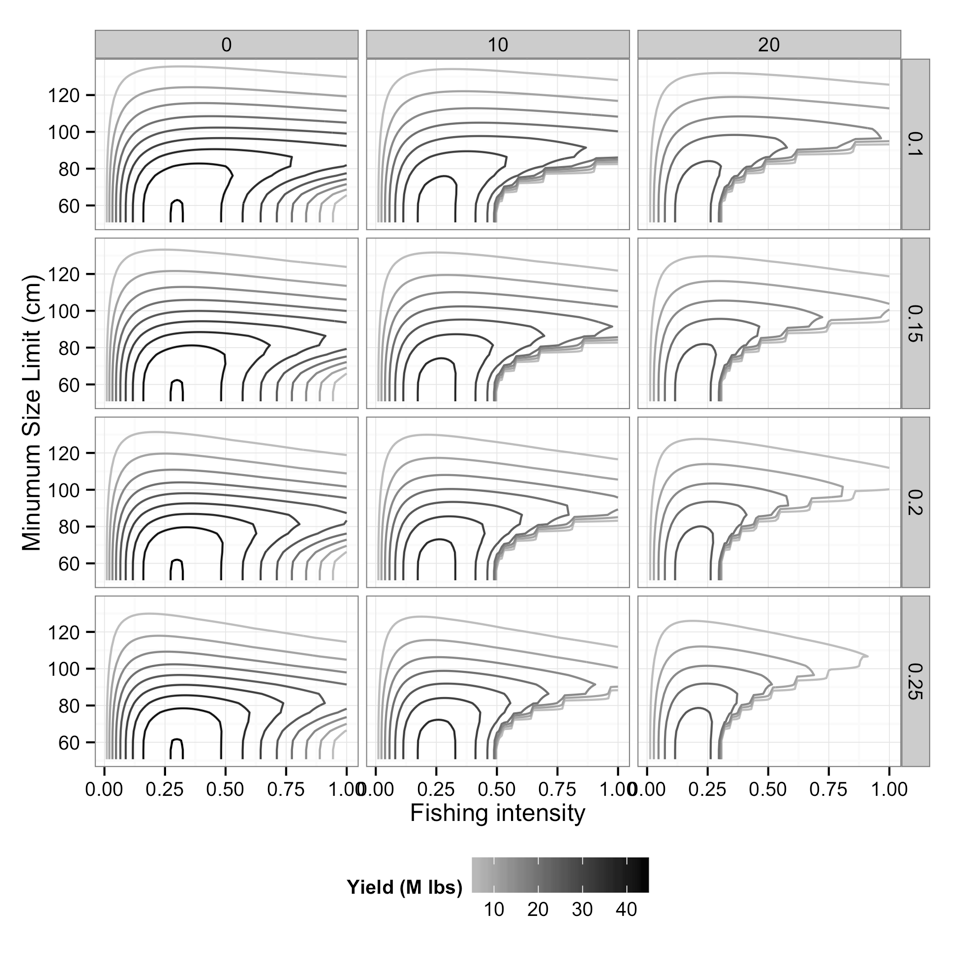
\includegraphics[width=\textwidth]{../figs/EquilibriumYield.png}
	\caption{Equilibrium yield isopleths for various combinations of fishing mortality rates and minimum size limits. Three columns represent bycatch caps of 0, 10 and 20 million pounds. Each row corresponds to discard mortality rates in the directed fishery of 0.10, 0.15, 0.2, and 0.25 per year.  Grey shading of each contour line represents total equilibrium catch in the directed fishery. }\label{fig:EquilibriumYield}
\end{figure}

\begin{figure}
	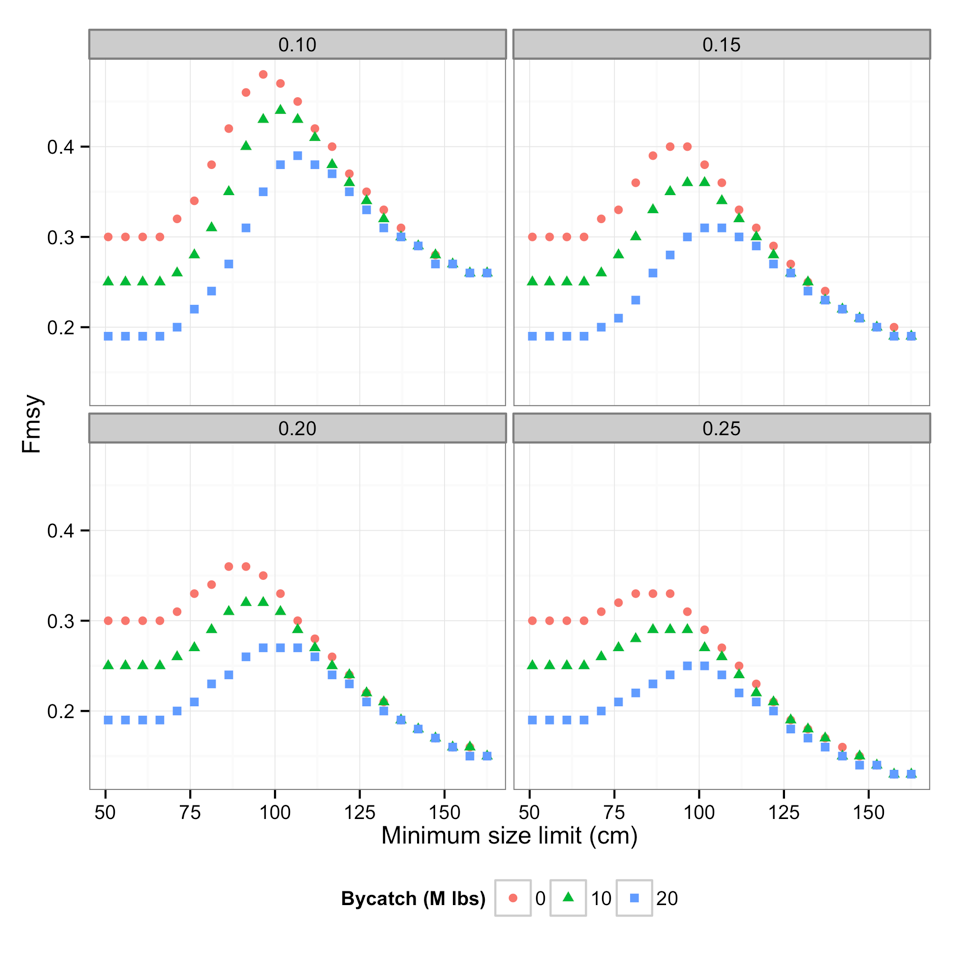
\includegraphics[width=\textwidth]{../figs/Fmsy.png}
	\caption{Estimates of \fmsy\ versus alternative minimum size-limits and three levels of bycatch. Each panel represents an alternative discard mortality rate (indicated on the top of the panel).}\label{fig:Fmsy}
\end{figure}



Lowering the minimum legal size-limit from 82 cm (32 inches) to 66 cm (26 inches) results in a lower estimate of \fmsy, and a much lower average weight of the catch (Table \ref{tab:MSY_reference_points}). The overall yield from the fishery is expected to increase with a lower size limit and the expected retained CPUE would also increase due to both increased legal biomass and the reduced amount of effort required to obtain the annual total allowable catch (TAC).  However, lowering the size limit raise some conservation concerns.  Estimates of \bmsy\ under a 66 cm size limit is lower due to increased fishing mortality rates required to achieve maximum sustainable yields.  Note also that under the lower size limit, estimates of \fmsy\ are all similar over alternative discard mortality rates and only differ relative to the amount of bycatch taken.  Under the lower size limit, the estimated selectivity for the directed fishery catches very few fish that are below the legal size-limit, and nearly all of the fish captured are retained (hence the insensitivity to discard mortality rates).

% %latex.default(t2)%
% %latex.default(t2)%
\begin{table}[!tbp]
\caption{Estimated MSY-based reference versus minimum size-limit (26 inch and 32 inch), discard mortality rates, bycatch levels of 0 and 10 million pounds, and the average weight of the catch in the directed fishery. }\label{tab:MSY_reference_points}
\begin{center}
\begin{tabular}{ccccccc}
\hline\hline
\multicolumn{1}{c}{Size}&
\multicolumn{1}{c}{Discard}&
\multicolumn{1}{c}{Bycatch}&
\multicolumn{1}{c}{}&
\multicolumn{1}{c}{}&
\multicolumn{1}{c}{MSY}&
\multicolumn{1}{c}{Average}
\tabularnewline
\multicolumn{1}{c}{limit}&
\multicolumn{1}{c}{mortality}&
\multicolumn{1}{c}{(M lbs)}&
\multicolumn{1}{c}{\fmsy}&
\multicolumn{1}{c}{\bmsy}&
\multicolumn{1}{c}{(M lbs)}&
\multicolumn{1}{c}{weight (lbs)}
\tabularnewline
\hline
$66.04$&$0.10$&$ 0$&$0.30$&$107.2$&$44.8$&$12.2$\tabularnewline
$66.04$&$0.10$&$10$&$0.25$&$110.0$&$36.5$&$12.5$\tabularnewline
$66.04$&$0.15$&$ 0$&$0.30$&$107.1$&$44.7$&$12.2$\tabularnewline
$66.04$&$0.15$&$10$&$0.25$&$109.8$&$36.4$&$12.5$\tabularnewline
$66.04$&$0.20$&$ 0$&$0.30$&$106.9$&$44.6$&$12.2$\tabularnewline
$66.04$&$0.20$&$10$&$0.25$&$109.6$&$36.3$&$12.5$\tabularnewline
$66.04$&$0.25$&$ 0$&$0.30$&$106.7$&$44.6$&$12.2$\tabularnewline
$66.04$&$0.25$&$10$&$0.25$&$109.4$&$36.3$&$12.5$\tabularnewline
\hline
$81.28$&$0.10$&$ 0$&$0.38$&$113.5$&$40.8$&$15.7$\tabularnewline
$81.28$&$0.10$&$10$&$0.31$&$116.7$&$33.5$&$16.4$\tabularnewline
$81.28$&$0.15$&$ 0$&$0.36$&$116.9$&$39.9$&$15.8$\tabularnewline
$81.28$&$0.15$&$10$&$0.30$&$118.0$&$32.8$&$16.5$\tabularnewline
$81.28$&$0.20$&$ 0$&$0.34$&$121.0$&$39.1$&$16.0$\tabularnewline
$81.28$&$0.20$&$10$&$0.29$&$119.6$&$32.1$&$16.6$\tabularnewline
$81.28$&$0.25$&$ 0$&$0.33$&$122.1$&$38.3$&$16.1$\tabularnewline
$81.28$&$0.25$&$10$&$0.28$&$121.5$&$31.5$&$16.7$\tabularnewline
\hline
\end{tabular}
\end{center}
\end{table}

Size-limits, discard mortality rates, and bycatch caps have a significant effect on the spawning potential ratio (Fig. \ref{fig:SPR}). Under steady-state conditions Spawning Potential Ratio (SPR) is also a measure of total mortality in the population.  The effect of imposing a minimum size-limit in the Pacific halibut fishery has the desired conservation effect of increasing spawning biomass for a fixed fishing mortality rate.  However, with increasing discard mortality rates, SPR values are reduced for a given size-limit and fishing mortality rate.  For example, with low discard mortality rates of 0.1 and a size-limit of 82 cm, the SPR=0.3 isopleth reaches a horizontal asymptote with increasing fishing mortality rate (Fig. \ref{fig:SPR}, upper left panel). However, as discard mortality rates increase, the conservation of spawning biomass diminishes as shown by the SPR isopleths turning upwards towards a vertical asymptote.  In other words, under conditions of high discard mortality rate, fishing effort must be reduced in order to maintain the same level of mortality as measured by the SPR.

Increasing levels of bycatch caps exacerbate the total mortality as measured by SPR (Fig. \ref{fig:SPR}).  For example, 10 million pounds of bycatch reduces the F$_{\textnormal{SPR=30}}$ from 0.3, to 0.24 in the absence of any size limit.  Increasing bycatch cap levels results in decreasing F$_{\textnormal{SPR=30}}$.

\begin{figure}
	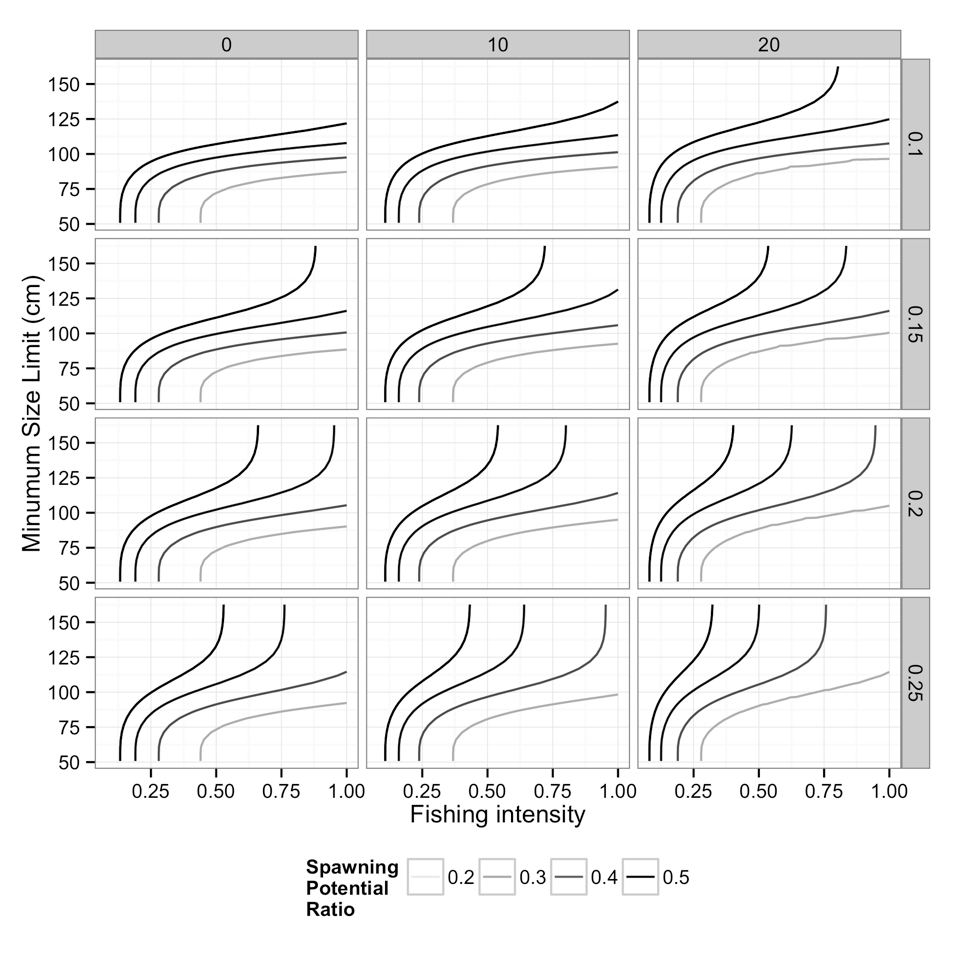
\includegraphics[width=\textwidth]{../figs/SPR.png}
	\caption{Isopleths for Spawning Potential Ratio (SPR) for combinations of fishing mortality, minimum size limit, discard mortality rates (rows) and bycatch caps of 0, 10, and 20 million pounds (columns).  }\label{fig:SPR}
\end{figure}

Relative economic losses associated with bycatch, size-limits, and discard mortality rates are based on the following arbitrary price schedule: 10-20 pound fish are valued at \$6.75 per pound, 20-40 pound fish at \$7.30 per pound, and fish greater than 40 pounds are valued at \$7.50 per pound.  In the bycatch fishery we assume no value for fish less than 10 pounds when evaluating the potential value of regulatory discards.

For the current minimum legal size-limit of 82 cm in the Pacific halibut fishery, the equilibrium yield versus directed fishing mortality and alternative bycatch rates and discard mortality rate are shown in Figure \ref{fig:YieldImpact}.  The relative effect of discard mortality rates in the directed fishery is relatively minor in comparison to the effects of bycatch in non-directed fisheries.  For example the difference in maximum sustainable yield (MSY) for the directed fishery with is roughly 2.5 million pounds over a range of discard mortality rates of 0.1 to 0.25.  The difference in landed value between the two discard mortality rates is roughly \$17 million and roughly \$20--\$23 million of halibut are discarded in the directed fishery in the form of sublegal fish  (Table \ref{tab:landedValue}).

The effects of bycatch from non-target fisheries are greater in terms of impacts on the maximum sustainable yield in the directed fisheries (Table \ref{tab:landedValue}).  A 10 million pound bycatch cap has the potential to reduce the average directed fisheries landings from 39.9 million pounds to 32.8 million pounds, assuming a discard mortality rate of 0.15 in the directed fishery.  This is roughly a 7.1 million pound loss in the directed fishery, which amounts to roughly a \$47 million dollar loss in the directed fishery in addition to the additional \$16 million loss associated with discarding sublegal fish.  Bycatch caps of 20 million pounds amount to a near \$100 million dollar loss in the directed fishery (Table \ref{tab:landedValue}).

\begin{table}[!tbp]
\caption{Estimates of MSY, \fmsy, for alternative discard mortality rates and bycatch levels assuming a minimum size-limit of 82 cm in the directed commercial longline fishery. Landed value is the expected landed value in the directed fishery. Discard value is the value of sub-legal halibut thrown overboard, and bycatch value is the value of halibut taken as regulatory discards that are discarded at sea.}\label{tab:landedValue}
\begin{center}
\begin{tabular}{lccccc}
\hline\hline
\multicolumn{1}{c}{Discard}&
\multicolumn{1}{c}{}&
\multicolumn{1}{c}{}&
\multicolumn{1}{c}{Landed}&
\multicolumn{1}{c}{Discard}&
\multicolumn{1}{c}{Bycatch}
\tabularnewline
\multicolumn{1}{c}{Mortality}&
\multicolumn{1}{c}{MSY}&
\multicolumn{1}{c}{\fmsy}&
\multicolumn{1}{c}{Value (millions)}&
\multicolumn{1}{c}{Value (millions)}&
\multicolumn{1}{c}{Value (millions)}
\tabularnewline
\hline
% $0.10$&$40.8$&$0.38$& \$276 & 23.7\tabularnewline
% $0.15$&$39.9$&$0.36$& \$270 & 22.4\tabularnewline
% $0.20$&$39.1$&$0.34$& \$265 & 21.1\tabularnewline
% $0.25$&$38.3$&$0.33$& \$260 & 20.3\tabularnewline
\multicolumn{6}{l}{No bycatch} \tabularnewline
$0.10$ & $40.8$ & $0.38$ & $276$ & $23$ & $ 0.0$\tabularnewline
$0.15$ & $39.9$ & $0.36$ & $270$ & $22$ & $ 0.0$\tabularnewline
$0.20$ & $39.1$ & $0.34$ & $265$ & $21$ & $ 0.0$\tabularnewline
$0.25$ & $38.3$ & $0.33$ & $260$ & $20$ & $ 0.0$\tabularnewline
\hline
\multicolumn{6}{l}{10 million pounds of bycatch} \tabularnewline
$0.10$ & $33.5$ & $0.31$ & $228$ & $16$ & $ 7.5$\tabularnewline
$0.15$ & $32.8$ & $0.30$ & $223$ & $16$ & $ 7.4$\tabularnewline
$0.20$ & $32.1$ & $0.29$ & $219$ & $15$ & $ 7.4$\tabularnewline
$0.25$ & $31.5$ & $0.28$ & $215$ & $14$ & $ 7.4$\tabularnewline
\hline
\multicolumn{6}{l}{20 million pounds of bycatch} \tabularnewline
$0.10$ & $25.6$ & $0.24$ & $176$ & $10$ & $14.1$\tabularnewline
$0.15$ & $25.1$ & $0.23$ & $173$ & $10$ & $14.0$\tabularnewline
$0.20$ & $24.7$ & $0.23$ & $170$ & $10$ & $13.9$\tabularnewline
$0.25$ & $24.2$ & $0.22$ & $167$ & $ 9$ & $13.9$\tabularnewline
\hline
\end{tabular}
\end{center}
\end{table}

\begin{figure}
	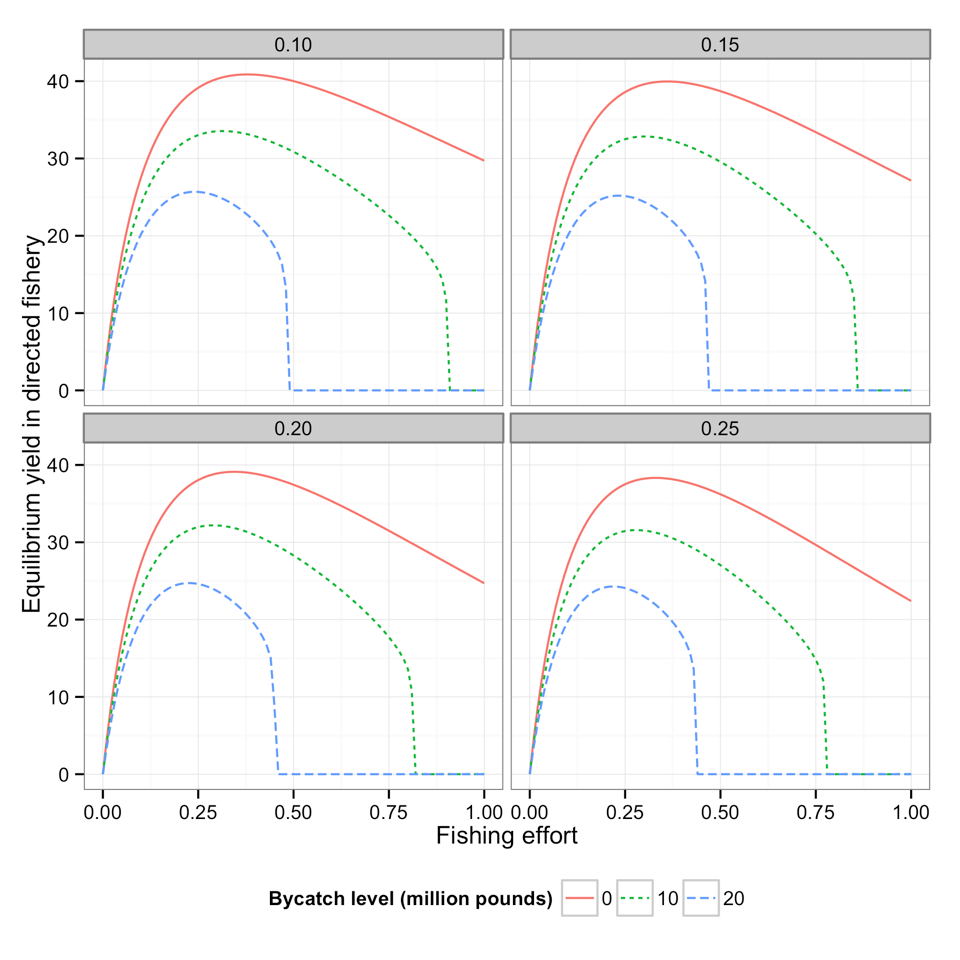
\includegraphics[width=\textwidth]{../figs/YieldImpact.png}
	\caption{Equilibrium yield in the directed fisheries under four alternative hypotheses about discard mortality rates (0.1, top left, 0.15, top right, 0.2, bottom left, and 0.25 bottom right) and a minimum legal size limit of 82 cm. On each panel, alternative ranges of bycatch from 0, to 20 million pounds are represented by alternative line types.}\label{fig:YieldImpact}
\end{figure}


\section*{Discussion}

Management of the Pacific halibut fishery poses many challenges for both analyst and decision makers with respect to utilizing the resource in a responsible and efficient manner.  Limits on annual total catches in the directed fisheries for halibut, including commercial long-line, sport and charter groups, food social and ceremonial fisheries, as well as personal use are determined each year by the International Pacific Halibut Commission (IPHC).  Bycatch limits and specifically prohibited species caps are ultimately set by other regulatory agencies including the North Pacific Fisheries Management Council, Pacific Fisheries Management Council and the Department of Fisheries and Oceans in Canada.  This arrangement puts the tradeoff between allocation for retained use and bycatch utilization in multiple agencies. Communication between these agencies is paramount to moving forward with developing harvest policies for Pacific halibut.

In this paper our overarching objective was to address the operational efficiency of the directed halibut fishery, and we hope that we have conveyed the message that this efficiency is related to both how the directed fisheries prosecute halibut in terms of understanding the tradeoffs between size-limits and  discard mortality rates of sub-legal fish.  In addition, bycatch caps in non-directed fisheries also play a significant role in determining optimal harvest rates and appropriate harvest control rules for managing the directed halibut fisheries.  Traditional use of MSY or SPR-based proxies for MSY related reference points are largely carried out using only information from the directed fisheries and rarely take into consideration the role of bycatch caps and discard mortality rates play in determining sustainable harvest policies.

The first specific objective to understand is how do size-limits and discard mortality rates influence reference point calculations in the directed fisheries.  The results of this paper are not that dissimilar of \cite{coggins2007ecm}, where increasing the minimum size-limit and increases in discard mortality rates substantially decreases the efficacy of protecting spawning biomass due to increased overall total mortality associated with increases in fishing effort required in order to obtain a fixed quota.  Spawning Stock Biomass per recruit is a measure of life-time reproductive potential and is a good measure of the reproductive potential of the stock.  The Spawning Potential Ratio (SPR) is a measure of fished to unfished reduction in the spawning potential and is often used as a proxy for fishing mortality, especially in cases where there are multiple fisheries that impact the same stock. Increasing the minimum size limit does preserve the SPR; however, increases in bycatch and discard mortality rates reduce the overall efficacy of using minumum size limits to guard against the potential of recruitment overfishing \citep{pineiii2008car}.

Another concern in the directed Pacific halibut fishery has been the recent reductions in mean size-at-age \citep{clark1999decadal,martell2013:ohr}.  Reduced growth rates and corresponding reductions in the mean size-at-age alone results in shifts towards lower yields and lower estimates of \fmsy\ in MSY-based reference point calculations.  One of the key features not fully explored in this model is the cumulative effects of size-selective fishing on halibut reference points and changes in the mean size-at-age for this stock.  The current harvest policy used by the IPHC was developed around the concept of density dependent growth; however, there are a number of other competing hypotheses that exist to explain the recent reductions in size-at-age for Pacific halibut.  \cite{sinclair2002disentangling} have look more carefully at this issue for Atlantic cod in the Gulf of St Lawrence and found that the primary effect of reductions in size-at-age was due to variation in size-selective mortality in the directed fisheries, but also noted that a combination of selective fishing, density-dependent growth and bioenergetic effects associated temperature difference also play a role.  In spite of what the underlying mechanism is for change in halibut size-at-age, fisheries efficiency decreases with reductions in size-at-age due to the minimum size-limits \citep{clark1995re}.  The effects is even more pronounced in the Gulf of Alaska where the current size-at-age is small in comparison to other regulatory areas \citep{Stewart2014}.

The equilibrium age-structured model used in this analysis is markedly different that previous models used to address harvest policy for the Pacific halibut fishery.  Previous models explicitly modeled the fate of 26-inch and larger halibut.  Bycatch and wastage of Pacific halibut less that 26-inches were not taken into direct consideration.  Until recently (2013), the assessment model for Pacific halibut only accounts for fish that are of age-6 and older \cite{clark2006assessment}; the vast majority of these age-classes are greater than 26 inches. Under 26 inch mortality associated with bycatch was deducted from the estimate of age-6 recruits and therefore changes in the under 26 inch bycatch levels had no impact on the harvest policy advice because these numbers would be soaked up in the annual estimates of recruitment.  The equilibrium model herein is based on all age- and size-classes, and hence an increase in under 26 inch bycatch in trawl fisheries more accurately represents the impacts on MSY and SPR-based reference points.

Lastly, the economic implications in this paper are based on a subjective price schedule that is very much a dynamic variable that changes from year to year.  We use these values merely to explore the impacts of bycatch and wastage on both the relative landings and potential value in the directed fishery.  These dollar amounts do not likely reflect the absolute values, but merely illustrate that a small loss due to bycatch (e.g., \$14 million dollars of halibut discarded in the trawl fishery under the 20 million pound bycatch cap) add up to significant losses in the directed fishery (e.g., roughly a \$100 million dollar loss to the directed fishery).  Traditionally, bycatch mitigation has only really examined the loss ratios of bycatch:catch, which are on the order of 1 pound of bycatch (26+ inch) translates into 1 pound of (32+ inch) loss to the directed fishery; the same ratio from a dollar perspective is on the order of 1.4:10.

\section*{Acknowledgements}

We greatly appreciate discussions with members of the IPHC Management Strategy Evaluation Board, and feedback from Robyn Forrest, Bruce Leaman and Jim Ianelli. The first author is hugely indebted to Carl J. Walters for the idea of capturing the cumulative effects of size-selective fishing in this model.


\addcontentsline{toc}{section}{References}
\bibliographystyle{apalike}
\bibliography{$HOME/Documents/ARTICLES/Articles-1}

\appendix
% \input{./Appendix/Growth}
%\input{./Appendix/F_ReferencePoints}

\end{document}
